\documentclass{IEEEtran}
\usepackage{cite}
\usepackage{authblk}
\usepackage{hyperref}
\usepackage{graphicx}
\usepackage{textgreek}

\graphicspath{{images/}}

\newcommand{\mailtodomain}[1]{\href{mailto:#1@nu.edu.kz}{\nolinkurl{#1}}}
\setlength{\parskip}{1em}

\begin{document}

\title{Engine mounts inspection using phase-based video magnification}

\author[1]{Anuar Maratkhan}
\author[2]{Kudaibergen Urinbayev}
\author[1]{Ibrakhim Ilyassov}
\affil[1]{Department of Computer Science}
\affil[2]{Department of Robotics and Mechatronics}
\affil[1,2]{Nazarbayev University \protect\\
53 Qabanbay Batyr Ave., 010000 \protect\\
Astana, Kazakhstan \protect\\
Email: \texttt{\{\mailtodomain{anuar.maratkhan}, \mailtodomain{kudaibergen.urinbayev}, \mailtodomain{ibrakhim.ilyassov}\}@nu.edu.kz}}

\maketitle

\begin{abstract}
Human visual system has some limitations. While human can recognize some vivid oscillations such as leave swings on the wind, some of subtle fluctuations like pulse or sway of bridge left unperceivable for the naked eye. However, small changes in motion could contain essential information of the system and could be quantitively and qualitatively analyzed. These analysis are done through a video magnification that we are applying for engine mount inspection in our work.
\end{abstract}

\section{Introduction}

Human visual system has some limitations. While human can recognize some vivid oscillations such as leave swings on the wind, some of subtle fluctuations like pulse or sway of bridge left unperceivable for the naked eye. However, small changes in motion could contain essential information of the system and could be quantitively and qualitatively analyzed. These analysis are done through a video magnification that we are applying for engine mount inspection in our work.

Several video magnification techniques were proposed. In 2005, Lie et al suggested Lagrangian approach to amplify motions in which pixels are tracked and motion vectors are amplified directly to synthesize videos with larger motions. This method required motion segmentation and manual correction of filling the holes after video processing \cite{Liu:2005:MM:1073204.1073223}.

Further, in 2012 new magnification method was proposed that used Eulerian approach. Eulerian Video Magnification (EVM) – computational method of video amplification of subtle motions and color changes over time \cite{Wu:2012:EVM:2185520.2185561}. The method saves large computational resources required in Lagrangian method of video magnifiying. However, the EVM method has some limitations due to its linearity. The method magnifies \textbf{all} motions in spatial domain, and thus, also magnifies the noise being present in the video.

A year later, \cite{Wadhwa:2013:PVM:2461912.2461966} discovered a method of the non-linear video magnification based on phase amplification in local sub-bands. By temporal filtering, the proposed method does not magnify noise, and therefore, makes possible to magnify video motions more. The method is based on obtaining spatial frequency sub-bands using Complex Steerable Pyramids, and further temporal filtering using bandpass filter. Then, we can amplify the certain phases which are motions in the video. Therefore, phase-based method was chosen for our work.

Above video magnification methods could be applied in several areas:

\begin{itemize}
	\item{Vital sign monitoring \cite{Aubakir2016VitalSM}}
	\item{Civil infrastructure}
	\item{Engine mount inspection}
\end{itemize}

The last application, in particular, will be used in our video magnification work. By comparing subtle vibrations in video sequence of engine of just manufactured car with the video of engine with properly working motor mount the defects of components could be detected. Thus, if the root-mean-square deviation (RMSE) of two videos exceeding appropriate threshold, this means more rigorous inspection is required and some mount flaws may exist in the system.

Similar works on car engine inspection using motion magnifications were not found. Therefore, this work has some novelty and may be advantageous for the car manufacturers.

\section{Background}

\subsection{Complex Steerable Pyramids}
The steerable pyramid \cite{119725} is an overcomplete transform that decomposes an image according to spatial scale, orientation, and position. We understand this work as a way to do local Fourier transform for certain bandpassed frequencies.

\subsection{Phase-based Video Magnification}
The steerable pyramid method mentioned above is used to measure local amplitude and phase, which are exploit in \cite{Wadhwa:2013:PVM:2461912.2461966} to process motion. Those phases are then magnified by $\alpha$.

These works are replicated in our work for further use in engine mount test through video magnification that is unseen to the naked eye. 

\section{Experimental setup}

The original setup for video capturing of car engine is shown on figure \ref{fig:setup}. For video shooting we need that gimbal to stabilize our motion that may result in additional noise in consequence. Although \cite{Wadhwa:2013:PVM:2461912.2461966} have used 400 fps camera to capture the engine working, the camera to be used in our work is iPhone 6 (or 7) camera with 240 fps in slow-motion video shooting.

\begin{figure}[h]
	\centering
	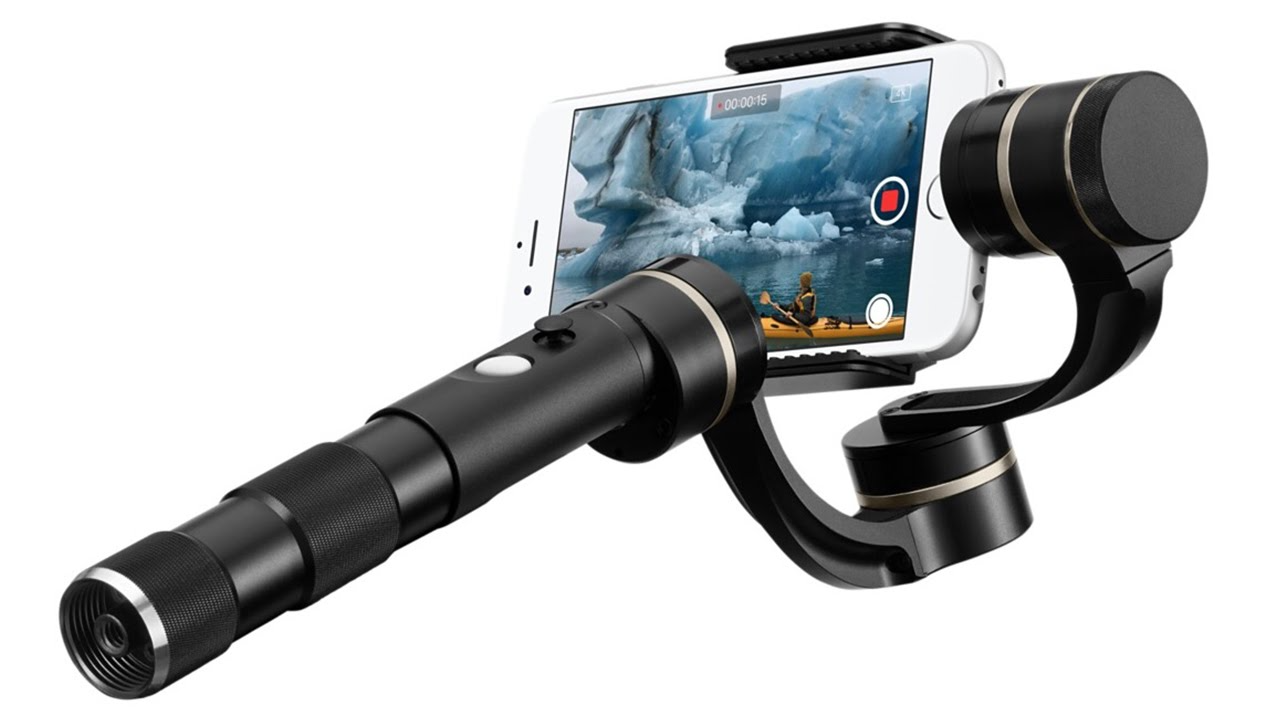
\includegraphics[width=0.5\textwidth]{maxresdefault}
	\caption{Controllable action camera gimbal}
	\label{fig:setup}
\end{figure}

Even though the video we are going to use is not filmed yet \footnote{Due to high load of students with final exams}, we used the video of \cite{Wadhwa:2013:PVM:2461912.2461966} with car engine as a sample for our experiments.

\begin{figure}[h]
	\centering
	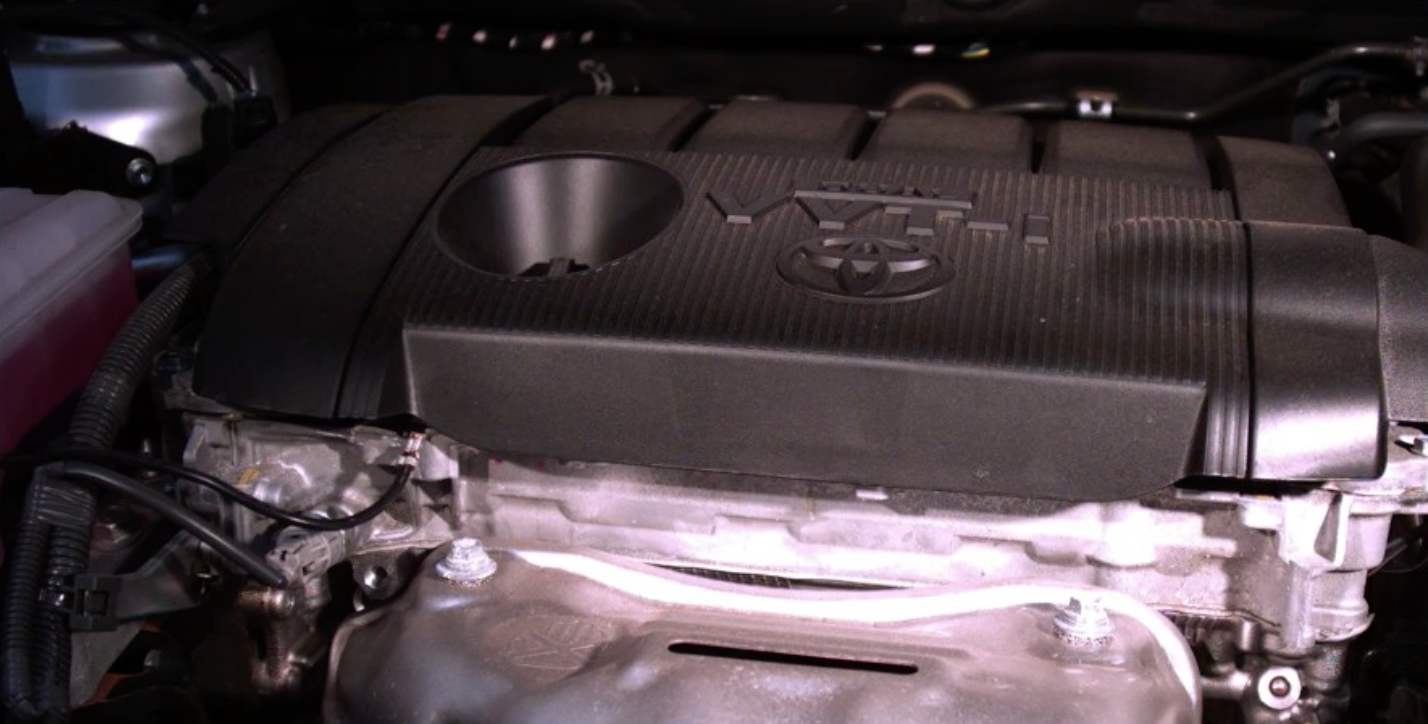
\includegraphics[width=0.5\textwidth]{car_engine}
	\caption{First frame of the sample video}
	\label{fig:engine}
\end{figure}

\section{Video Magnification}

The above mentioned sample video has been motion magnified using the existing code base of \cite{Wadhwa:2013:PVM:2461912.2461966} in MATLAB. For any video to be motion magnified we need to provide:

\begin{itemize}
	\item{video sequence in high fps}
	\item{high and low subband frequencies to be bandpassed}
	\item{$\alpha$ coefficient to magnify obtained phases.}
\end{itemize}

Our first mistake was to use low fps (30 fps) video sequence for motion magnification. The output of the magnification was unsuccessful. Thus, we need high fps camera to shoot the engine.

The high and low band frequencies are needed to bandpass frequencies in that range for further phase magnification. The original work of \cite{Wadhwa:2013:PVM:2461912.2461966} has used 15 Hz for low and 25 Hz for high band frequencies. The same was applied in our experiments.

The $\alpha$ coefficient is used to magnify the motion for such amount. The higher the $\alpha$, the more the motion is magnified. We used $\alpha$ equal to 15 in our experiments, as was used in \cite{Wadhwa:2013:PVM:2461912.2461966}.

\section{Conclusion}

To conclude, the most work done is a replication of \cite{Wadhwa:2013:PVM:2461912.2461966} study for engine mount inspection. There is still work to be done with conversion of existing code base to Python code with frequent usage of OpenCV and NumPy libraries.

\bibliographystyle{IEEEtran}
\bibliography{reference}
\printbibliography

\end{document}